%Pakete;
%A4, Report, 12pt
\documentclass[ngerman,a4paper,12pt]{scrreprt}
\usepackage[a4paper, right=20mm, left=20mm,top=20mm, bottom=30mm, marginparsep=5mm, marginparwidth=5mm, headheight=7mm, headsep=15mm,footskip=15mm]{geometry}

%Papierausrichtungen
\usepackage{pdflscape}
\usepackage{lscape}

%Deutsche Umlaute, Schriftart, Deutsche Bezeichnungen
\usepackage[utf8]{inputenc}
\usepackage[T1]{fontenc}
\usepackage[ngerman]{babel}

%quellcode
\usepackage{listings}

%tabellen
\usepackage{tabularx}

%listen und aufzählungen
\usepackage{paralist}

%farben
\usepackage[svgnames,table,hyperref]{xcolor}

%symbole
\usepackage{latexsym,textcomp}

%font
\usepackage{helvet}
\renewcommand{\familydefault}{\sfdefault}

%Abkürzungsverzeichnisse
\usepackage[printonlyused]{acronym}

%Bilder
\usepackage{graphicx} %Bilder
\usepackage{float}	  %"Floating" Objects, Bilder, Tabellen...
\usepackage[space]{grffile} %Leerzechen Problem bei includegraphics
\usepackage{wallpaper} %Seitenhintergrund setzen
\usepackage{transparent} %Transparenz

%for
\usepackage{forloop}
\usepackage{ifthen}

%Dokumenteigenschaften
\title{Repetitionsfragen CN1}
\author{Tobias Blaser}
\date{\today{}, Rapperswil}


%Kopf- /Fusszeile
\usepackage{fancyhdr}
\usepackage{lastpage}

\pagestyle{fancy}
	\fancyhf{} %alle Kopf- und Fußzeilenfelder bereinigen
	\renewcommand{\headrulewidth}{0pt} %obere Trennlinie
	\fancyfoot[L]{Seite \thepage/\pageref{LastPage}} %Fusszeile mitte
	\fancyfoot[R]{\today{}} %Fusszeile rechts
	\renewcommand{\footrulewidth}{0.4pt} %untere Trennlinie

%Kopf-/ Fusszeile auf chapter page
\fancypagestyle{plain} {
	\fancyhf{} %alle Kopf- und Fußzeilenfelder bereinigen
	\renewcommand{\headrulewidth}{0pt} %obere Trennlinie
	\fancyfoot[L]{Seite \thepage/\pageref{LastPage}} %Fusszeile mitte
	\fancyfoot[R]{\today{}} %Fusszeile rechts
	\renewcommand{\footrulewidth}{0.4pt} %untere Trennlinie
}

\usepackage{changepage}

% Abkürzungen für Kapitel, Titel und Listen
%listen und aufzählungen
\usepackage{paralist}
\usepackage{mdwlist}

% list short cuts
\newcommand{\ul}{
	\begin{itemize}
}
\newcommand{\ulE}{
	\end{itemize}
}
\newcommand{\ol}{
	\begin{enumerate}
}
\newcommand{\olR}{
	\resume{enumerate}
}
\newcommand{\olE}{
	\end{enumerate}
}
\newcommand{\olS}{
	\suspend{enumerate}
}
\newcommand{\li}{
	\item
}
\newcommand{\dl}{
	\begin{description}
}
\newcommand{\di}[1]{
	\item[#1]
}
\newcommand{\dlE}{
	\end{description}
}
\newcommand{\ra}{
	$\rightarrow$
}

% chapter and section shortcuts
\newcommand{\ch}[1]{
	\chapter{#1}
}
\newcommand{\se}[1]{
	\section{#1}
}
\newcommand{\sse}[1]{
	\subsection{#1}
}
\newcommand{\sss}[1]{
	\subsubsection{#1}
}

%links, verlinktes Inhaltsverzeichnis, PDF Inhaltsverzeichnis
\usepackage[bookmarks=true,
bookmarksopen=true,
bookmarksnumbered=true,
breaklinks=true,
colorlinks=true,
linkcolor=black,
anchorcolor=black,
citecolor=black,
filecolor=black,
menucolor=black,
pagecolor=black,
urlcolor=black
]{hyperref} % Paket muss unbedingt als letzes eingebunden werden!

\usepackage{graphicx}
\begin{document}

% Titel, Inhaltsverzeichnis
\tableofcontents
\clearpage


\ch{Informationsverarbeitung \& Wahrscheinlichkeitsrechnung}

\se{Informationsverarbeitung}
\ol
	\li Erklären Sie das Modell der Informationsverarbeitung. Erklären Sie die Begriffe Kanal, Sender, Empfänger, Modulator, Demodulator, Kanal Coder, Quellen und Senken.
\olS

\se{Wahrscheinlichkeitsrechnung}
\olR
	\li Was ist ein Zufallsvorgang? Nennen Sie zwei wesentliche Punkte und nennen Sie drei Beispiele aus der Informatik.
	\li Erklären Sie die Ergebnis- und Ereignismenge eines Zufallsvorgangs. Geben Sie folgendes an:
		\ol
			\li Omega und Anzahl Ergebnisse des Zufallvorgangs „Werfen eines Würfels“.
			\li Omega und Anzahl Ergebnisse des Zufallsvorgangs „Werfen eines Würfels solange bis eine 6 kommt“.
		\olE
	\li Erklären und begründen Sie die Rechenregeln für Wahrscheinlichkeiten.
	\li Lösen Sie die folgende Aufgaben (Quelle: Folien Dozent) durch überlegen mittels Wenn-Diagramm und verifizieren Sie das Resultat durch rechnen: 
„In einer Stadt erscheinen 2 Lokalzeitungen, die Morgenpost und der Stadtspiegel. Die Wahrscheinlichkeit, dass ein bewohner der Stadt die MP liest ist 0.6, dass er den SS liesst 0.5 und dass er MP oder SS liest 0.9.“	
Wie gross ist die Wahrscheinlichkeit, 
		\ol
			\li dass jemand beide Blätter kauft?
			\li Dass jemand kein Blatt liest?
			\li Dass jemand genau eines der beiden Blätter liest?
		\olE
\olS


\ch{Informationsgehalt und Entropie}
\olR
	\li Erklären Sie das Modell der Informationsverarbeitung
	\li Wann ist eine Nachricht eine Information?
	\li Was ist der Entscheidungsgehalt einer Nachricht? Was ist der Informationsgehalt eines Zeichens? Wie berechnen Sie ihn?
	\li Was ist Entropie? Wie hängen Informationsgehalt, Elementarentscheidungen und Entropie zusammen?
	\li Was ist die mittlere Codewortlänge? Wie wird sie ermittelt?
	\li Was ist eine Präfixeigenschaft?
	\li Wie berechnen sie Redundanz von Code und Quelle?
	\li Was sind diskrete Quellen mit und ohne Gedächnis?
\olS


\ch{Komprimierungsverfahren}
\olR
	\li Welche drei Arten von Verfahren zur Datenkompression gibt es?
	\li Erklären Sie die Huffman Codierung. Machen Sie ein Beispiel.
	\li Wie funktioniert die Lempel-Ziv Codierung?
	\li Wie können Sie die Huffman Codierung und die Lempel-Ziv Codierung kombinieren?
\olS


\ch{Verschlüsselungsverfahren}
\olR
	\li Erklären Sie, was symetrische und asymetrische Verschlüsselungsverfahren sind.
	\li Erklären Sie, wie das Substitutionsverfahren, das Transpositionsverfahren, das Playfair-Chiffre Verfahren, und das Vigenàir-Chiffre Verfahren funktionieren und machen Sie zu jedem ein Beispeil.
	\li Erklären Sie, was die Rotormaschine, die Enigma und das DES sind, nach welchen Prinzipien sie funktionieren und wie entschlüsselungssicher sie waren.
	\li Wie berehnen Sie zu einer Zahl die inverse? Machen Sie ein Beipiel.
	\li Wie berechnen Sie zu zwei Zahlen den grössten gemeinsamen Teiler?
	\li Erklären Sie den inversen euklidischen Algorithmus.
	\li Erklären Sie, wie RSA funktioniert. Machen Sie ein Beispiel.
\olS


\ch{Informationstheorie und Kanalcodierung}
\olR
	\li Erklären Sie die Kanalmatrix.
	\li Was ist Transinformation?
	\li Was ist Verbundentropie?
	\li Was ist Äquivokation?
	\li Was ist Rauschen, was ist Irrelevanz?
	\li Erklären Sie den n-dimensionalen Coderaum.
	\li Aus welchem Grund wird Redundanz bewusst hinzugefügt?
	\li Erklären Sie die flachgedrückte Darstellung von n-dimensionalen Räumen.
	\li Was ist eine Korrigierkugel und für was wird sie verwendet? Was ist wenn die Korrigierkugeln einander nicht berühren, einander berühren, sich überlappen?
	\li Was ist die Hammingdistanz?
	\li Wann ist ein Coderaum dicht gepackt?
	\li Wie funktioniert der Hamming Code?
	\li Was ist das Fehlersyndrom?
\olS


\ch{Blockcodes und zyklische Codes}
\olR
	\li Wie bestimmen Sie zu einer Matrix die Hemmingdistanz?
	\li Woran erkennen Sie die Anzahl Kontrollstellen?
	\li Was ist das Fehlersyndrom und wie berechnen Sie es?
	\li Was ist ein zyklische Code? Wie ermitteln Sie die Anzahl Kontrollstellen?
	\li Wie funktioniert ein Schieberegister?
	\li Welche Eigenschaften besitzt der Abramson Code? Wie erkennen Sie, ob Ihnen ein Abramson-Code oder ein Hemming-Code vorliegt?
\olS


\ch{Faltungscodes}
\olR
	\li Was ist Faltung im Mathem. Sinne?
	\li Welche Vorteile bieten Faltungscodes gegenüber Blockcodes?
	\li Erklären Sie schematisch, wie ein Faltungscode Encoder funktioniert.
	\li Abb. \ref{encs}: Erklären Sie die Abbildung und zeichnen Sie das gleiche Schema für eine (3,1,2) und eine (1,1,2) Encoderschaltung (Erfinden Sie jeweils selbst Gleichungen für die Faltung). Zeichnen Sie zu jedem Encoder den zugehörigen DEA mit Übergängen und Output-Bits. Geben Sie zum gegebenen Encoder die Gleichungen des Faltungscodes an.
	\begin{figure}[H]
		\centering
		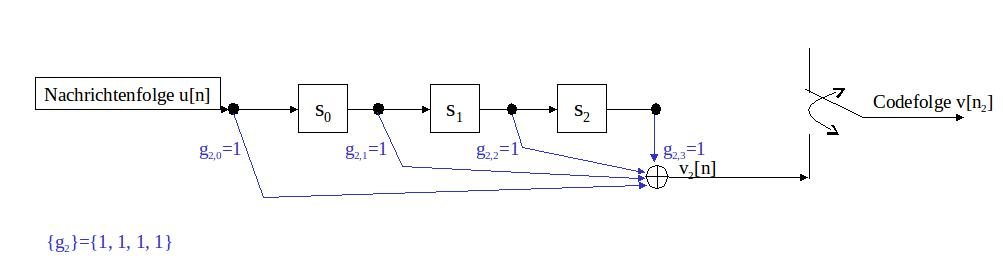
\includegraphics[width=\textwidth]{img/R7.1.jpg}
		\caption{}
		\label{encs}
	\end{figure}
	\li Was ist das Natz- oder Trellisdiagramm? Wie finden Sie darin den entsprechenden Pfad? Machen Sie dies am Beispiel der Figur \ref{encs}.
	\li Was bedeutet das "Gewicht" eines Codes und was ist der Fundamentalweg?
\olS


\ch{Einführung Signale}
\olR
	\li Was ist "intrinsische Information"?
	\li Welche Kenngrössen definieren ein Signal?
	\li Erklären Sie, was ein dB ist. 
	\li Was passiert, wenn harmonische Signale addiert werden?
	\li Erklären Sie, was es bedeutet, ein Signal in seine Spektralanteile zu zerlegen.
	\li Was passiert mit einem akkustischen Signal, wenn Sie die Phase positiv verändern?
	\li Was passiert mit einem akkustischen Signal, wenn Sie die Frequenz erhöhen?
	\li Was passiert mit einem akkustischen Signal, wenn Sie die Periodendauer verkürzen?
	\li Was passiert mit einem akkustischen Signal, wenn Sie die Amplitude vergrössern?
	\li Warum besteht ein Rechtecksignal aus ganz vielen verschiedenen Frequenzen? Machen Sie ein Beispiel und zeichnen Sie das Signal sowohl in einem Zeit wie auch in einem Frequenzdiagramm (grob).
	\li Wie können Sie ein Geräusch orten? Was macht ihr Gehirn?
\olS

\olR
	\li Wie hören sich Signale gleicher Form aber unterschiedlicher Phase an? Warum?
	\li Wie hören sich Signale unterschiedlicher Form aber gleicher Frequenz an? Warum?
	\li Welchen Einfluss hat ein Filter?
	\li Wie verändert sich ein Signal, wenn ich verschiedene Filter darauf anwende?
		\ul
			\li Sinus
			\li Rechteck
			\li Dreieck
			\li Sägezahn
		\ulE
	\li Kann durch eine Filterbank ein beliebiges Signal in seine Spektralanteile zerlegt werden?
	\li Was passiert, wenn harmonische Signale addiert werden?
	\li Was passiert, wenn harmonische Signale multipliziert werden? Was passiert, wenn, wenn zwei solche Signale wieder multipliziert werden? Welche Rolle spielt die Phase?
	\li Was ist Frequenzmultiplex?
	\li Was ist ein Tiefbass, was ein Hochbass? Was ein Basisband?
	\li Wie wird bei der Multiplikation zweier Signale das ursprüngliche Signal zurückgewonnen werden? Wie wird dabei eine Phasenverschiebung verhindert?
\olS

\ch{Sprache}
\olR
	\li Was bedeuten Abtastung und Quantisierung in Bezug auf die Digitalisierung und Übertragung von Sprache?
	\li Wie kann ein analoges Sprachsignal abgetastet werden? Wie wirkt sich dies auf den Frequenzbereich aus?
	\li Abb. \ref{zeitdiskret}: Erklären Sie die folgende Grafik:
	\begin{figure}[H]
		\centering
		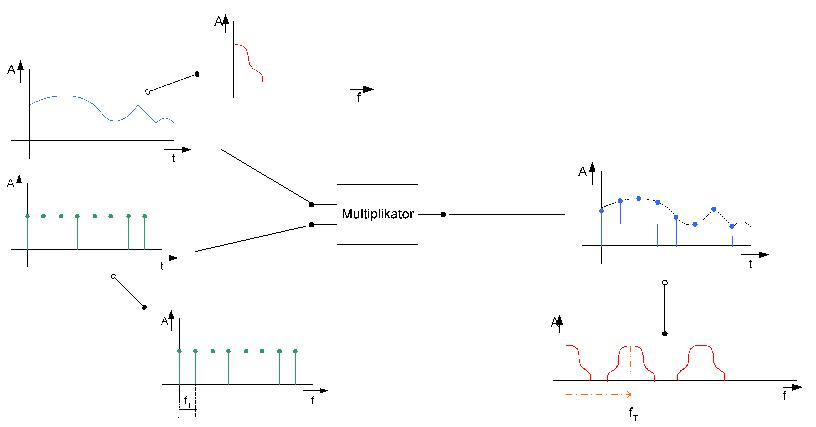
\includegraphics[width=\textwidth]{img/R10.1.jpg}
		\caption{}
		\label{zeitdiskret}
	\end{figure}
	\li Wie erhält man aus dem abgetasteten Signal das Sprachsignal zurück?
	\li Erklären Sie, wie gross der Fehler ist, der durch die Zeitabtastung entsteht.
	\li Was bedeutet quantisieren? Was passiert dabei mit der Sprachinformation, was für ein Signal resultiert?
	\li Erklären Sie das prinzip der Kompression bei Sprache.
	\li Erklären Sie grob, was bei MPEG-1 zur Kompression von Audio Daten abläuft.
	\li Wie kann Sprache und dessen Sprecher erkannt werden?
\olS

\ch{Analog / Digital}
\olR
	\li Erklären Sie, was Quantisierung ist. Was für Signale können quantisiert werden?
	\li Was für ein Signal resultiert? Wie unterscheidet sich das Signal im Frequenzspektrum vom originalen Signal?
	\li Wie führen Sie ein quantisiertes Signal zurük zu akkustischer Sprache?
	\li Wie gross ist der bei der Quantisierung entstandene Fehler?
	\li Was ist Kompandierung? Was Expandierung? Erklären Sie wie die Kompression von Sprache funktioniert.
\olS

\ch{Signale als Träger vom Information}
\olR
	\li Warum soll ein Signal Gleichspannungsfrei sein?
	\li Was ist ein return-to-zero/non-return-to-zero Signal?
	\li Welche Signalabbildungsmöglichkeiten haben Sie, wenn Sie nur mit der Amplitude arbeiten? Welche Möglichkeiten kommen hinzu, wenn Sie noch die Phasenverschiebung nutzen?
	\li Wie können Sie bei einem mit Phasenverschiebung abgebildeten Signal 0 und 1 analysieren?
	\li Erklären Sie, welches Prinzip beim OFDM zur Anwendung kommt. Machen Sie eine Skizze. Kann man OFDM auch auf Sprache anwenden?	
	\li Machen Sie eine Skizze, wie ein Bitstrom  aufgetrennt und in vier Frequenzen gesplitted wird und anschliessend mit OFDM auf der Leitung aussieht. Zeichnen Sie auch logische Bausteine, wie z.B. Addierer ein.
\olS





\end{document}
